% oil_mc_pres.tex
\documentclass{beamer}
\usepackage{url} 
\usepackage{amsmath}
\usepackage{esdiff} %for writing partial derivatives

\usetheme{default}

\title[oil]{Estimating the Effect of Price on Oil Production: Evidence from the Norwegian Continental Shelf}
\author{
Johannes Mauritzen \\ 
NHH Norwegian School of Economics \\
jmaurit@gmail.com \\
\url{jmaurit.github.io\#oil\_prices}
% \url{jmaurit.github.io\\#oil\_prices}
}

\date{May 29th, 2015}

\begin{document}

%--- the titlepage frame -------------------------%
\begin{frame}[plain]
  \titlepage
\end{frame}

\begin{frame}[plain]
	Main Results
	\begin{itemize}
		\item Use of semi-parametric models can be used to make non-biased estimates of oil-field production.
		\item No significant contemporary effect of oil price on field production.
		\item Slight lagged effect found after 2-4 years, magnitude of around 2-5\%.
	\end{itemize}
\end{frame}


\begin{frame}
	\begin{figure}
	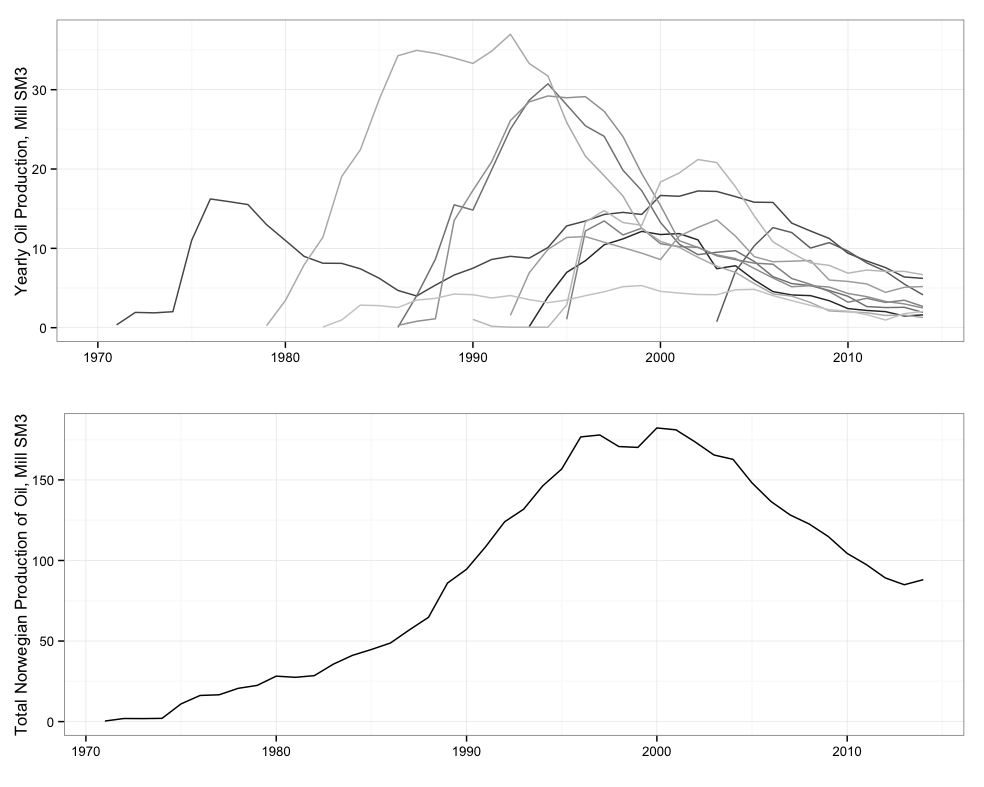
\includegraphics[width=1\textwidth]{figures/oil_decline.png}
	% \caption{The top panel shows the production from the largest 10 oil fields, whose starting times are temporally correlated with each other.  The total production over time is bell-shaped, as shown by the bottom panel.}
	\label{oil_decline}
\end{figure}
\end{frame}



\begin{frame}
\begin{figure}
	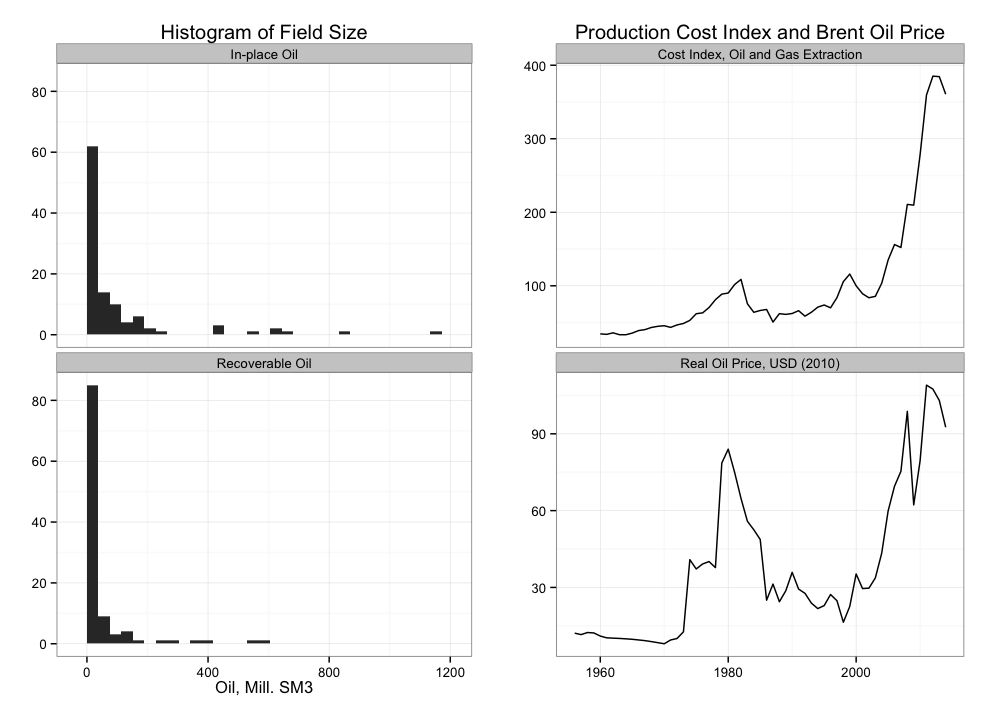
\includegraphics[width=1\textwidth]{figures/data_descriptives.png}
	% \caption{Data descriptives. The left panels show histograms of estimates of recoverable oil and in-place oil by field. The right panels shows the production cost index and real Brent oil prices.}
	\label{data_descriptives}
\end{figure}
\end{frame}



\begin{frame}
\begin{equation}
\begin{split}
	Log(production_{i,t}) & = f(production\_time_{i,t}) + f(year_t) + \beta_1 in\_place\_oil_{i,t}\\
	 \quad & + \beta_3 cost\_index_{t} + \mathbf{\beta_2 oil\_price\_lags_t} +  
	  \epsilon_{i,t}
\label{gam_price_eqn}
\end{split}
\end{equation}
\end{frame}


\begin{frame}
\begin{equation}
\| \mathbf{y} - \mathbf{X\beta} \| ^2 + \lambda \int_{0}^{1} [f^{\prime \prime}(x)]^2 dx
\label{min_equation}
\end{equation}
\end{frame}



\begin{frame}
\begin{figure}
	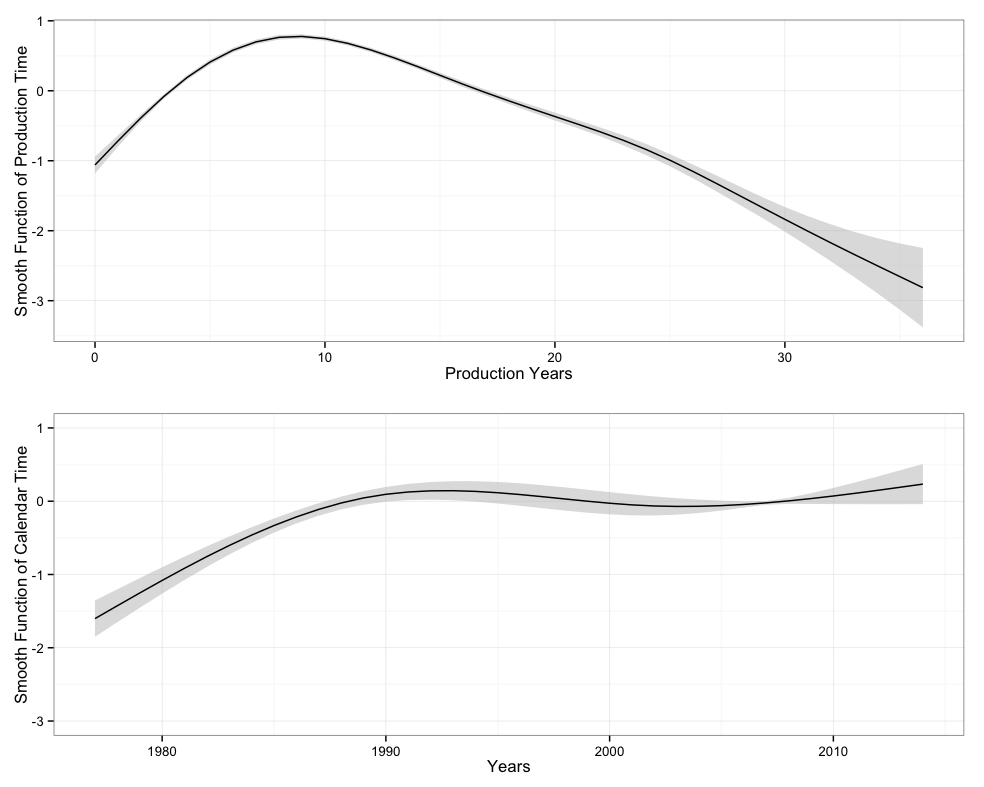
\includegraphics[width=1\textwidth]{figures/smooths.png}
	% \caption{The estimated smoothed functions over production time and calendar time.}
	\label{smooths}
\end{figure}
\end{frame}




\begin{frame}
	\begin{equation}
	y_i = g(x_1, x_2)
	\label{thin_plate_1}
	\end{equation}

	\begin{equation}
\min \|\boldsymbol{y-f}\|^2 + \lambda J_{22}(f)
\label{thin_plate_2}
	\end{equation}

\end{frame}



\begin{frame}
\begin{equation}
	J_{22}(f)= \Big(  \diffp[2]{f}{x_1} \Big)^2 +
	 \Big(\frac{\partial^2 f}{\partial x_1 \partial x_2}\Big)^2 + 
	\Big(\diffp[2]{f}{x_2} \Big)^2dx_1 dx_2
\label{thin_plate_3}
	\end{equation}
\end{frame}



\begin{frame}
	\begin{figure}
		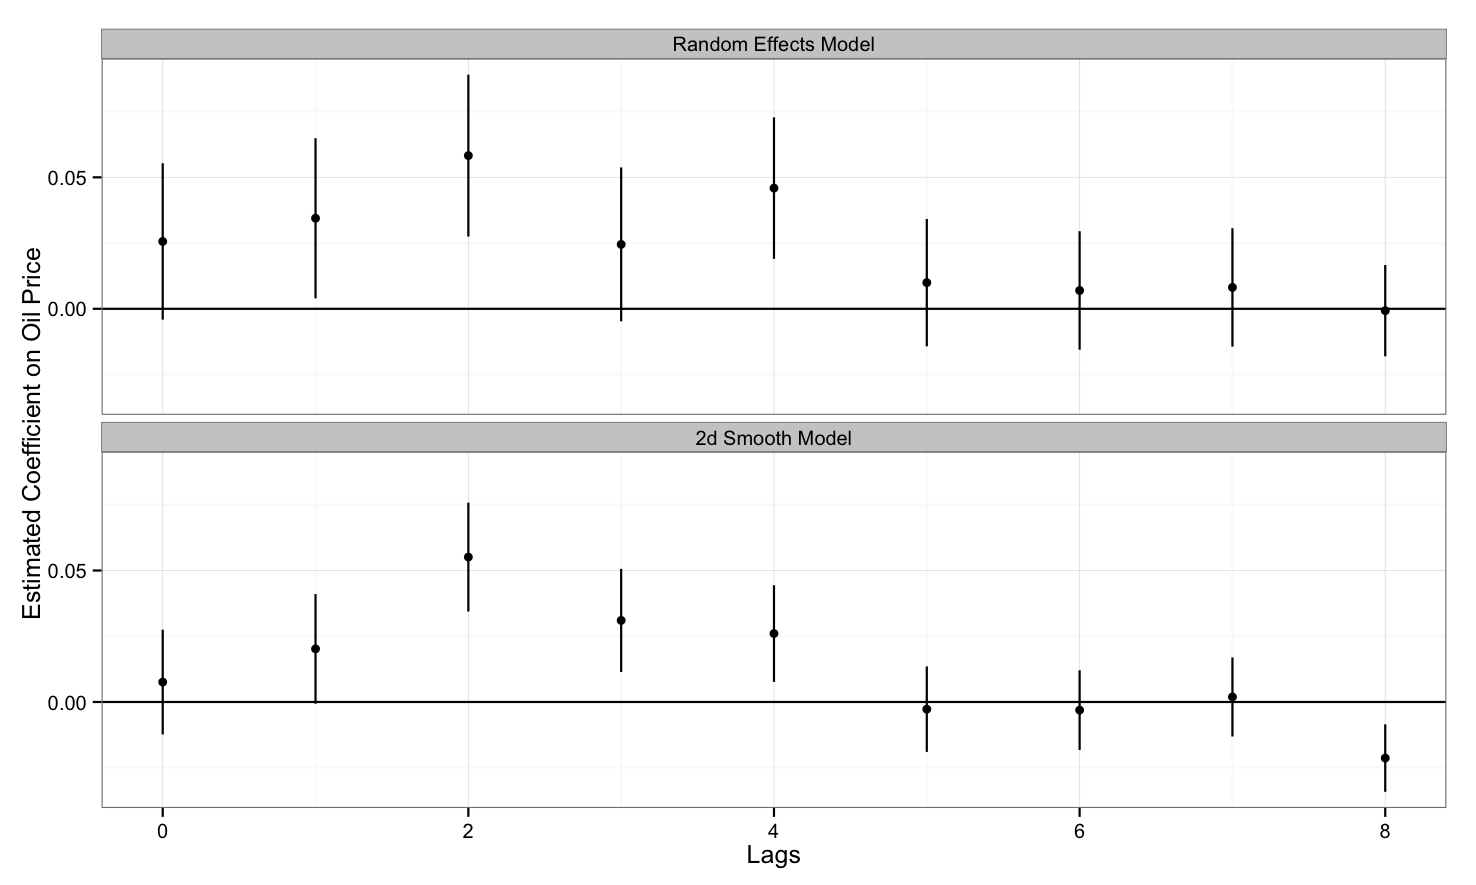
\includegraphics[width=1\textwidth]{figures/price_coefficents.png}
		% \caption{Estimated coefficients from two GAM models: a model with random field effects and single smoothed function of production time, and another with a two dimensional smoothed function of production time and field size.  The points represent the point estimates, while the lines represent approximate 95\% confidence intervals. Significant positive coefficients are estimated on lags of between 1-4 years.  However, little to no effect is measured on the concurrent price term.}
		\label{price_coefficients}
	\end{figure}
\end{frame}



\begin{frame}
	\begin{figure}
		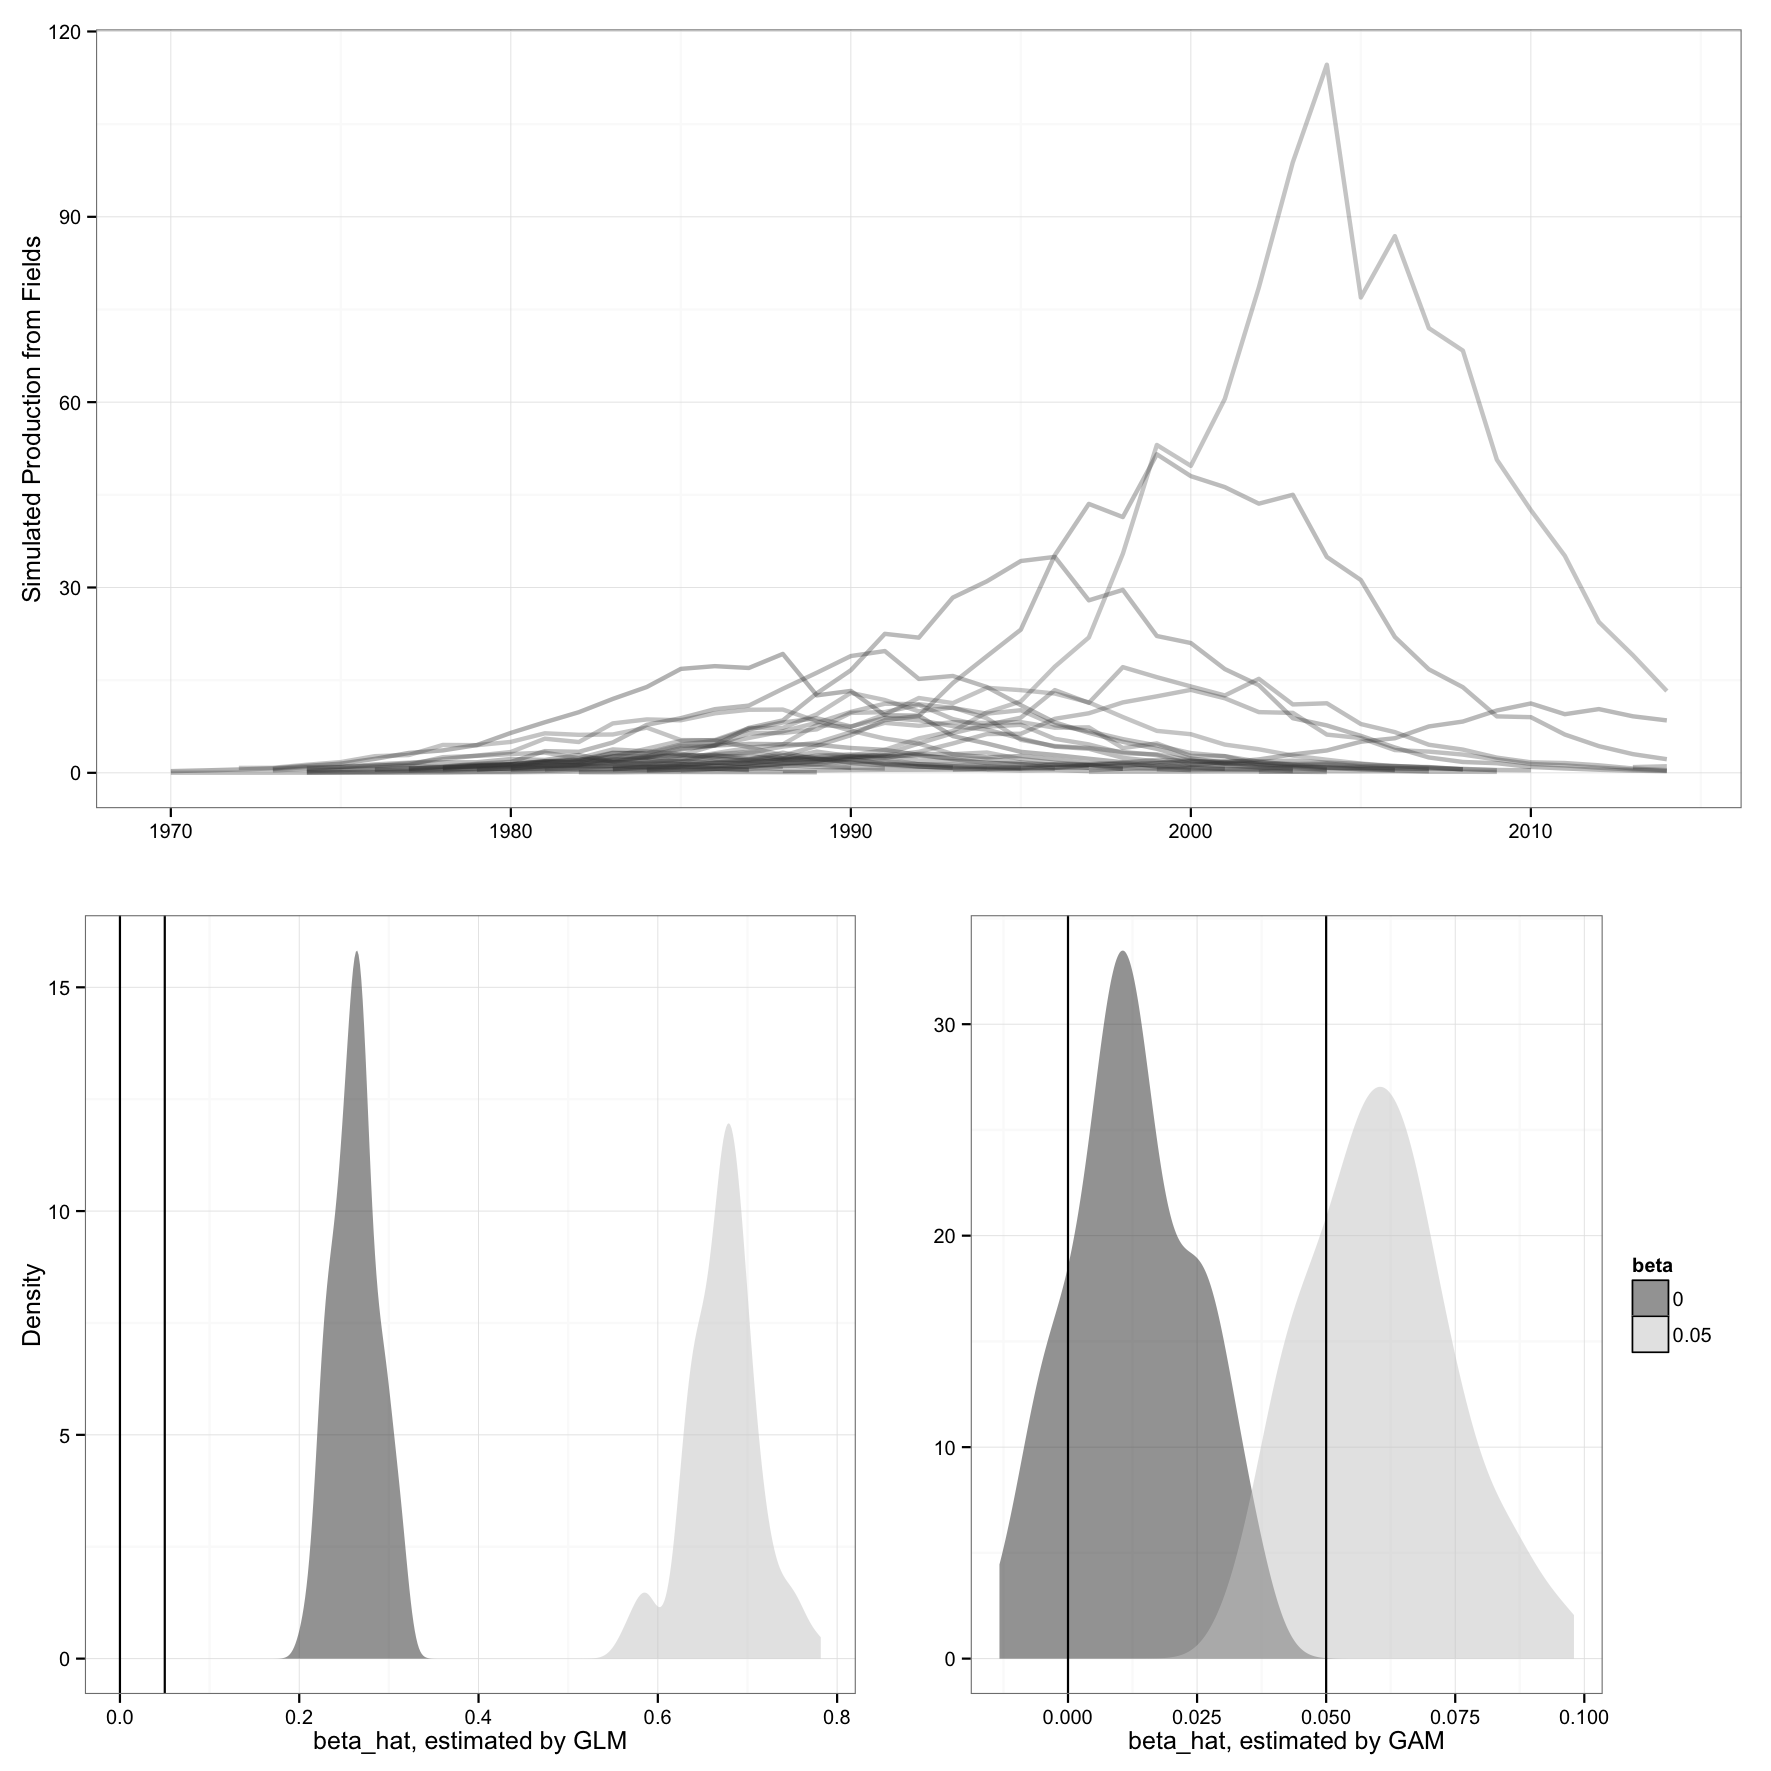
\includegraphics[width=.8\textwidth]{figures/mc_plot.png}
		% \caption{Results from a Monte-Carlo experiment. I generate data mimicking oil price production from a set of fields, as displayed in the top frame. Using GLM and GAM models, and regenerating the error component in the data, I replicate estimates of the effect of price on production, which is set at $\beta = 0$ and $\beta=0.05$. The density of the results for the GLM model are shown in the lower left panel, where a clear and large bias is shown relative to the true $\beta$ which are represented by the vertical lines.  A GAM model however provides estimates close to the true $\beta$}
		\label{mc_results}
	\end{figure}
\end{frame}


\begin{frame}[plain]
	Main Points
	\begin{itemize}
		\item Offshore producers are unlikely to be strategically adjusting production to short-term changes in the oil price
	\end{itemize}
\end{frame}

\begin{frame}[plain]
	Main Points
	\begin{itemize}
		\item Offshore producers are unlikely to be strategically adjusting production to short-term changes in the oil price
		\item Some investment-led lagged response likely, but of modest magnitude.
	\end{itemize}
\end{frame}

\begin{frame}[plain]
	Main Implications
	\begin{itemize}
		\item Oil production from exiting offshore fields inelastic to changes in oil prices.  
		\item Most of effect on total extraction from offshore areas likely comes from geographic and technical expansion.
	\end{itemize}
\end{frame}




\end{document}